\documentclass[a4paper,leqno,12pt]{amsart}
%
\usepackage{amsmath,amsthm}
\usepackage{graphicx}
\usepackage[margin=0.7in]{geometry}

\usepackage{enumitem}

\usepackage{multirow}
\usepackage{tikz}
\usepackage{wrapfig}

\usepackage{fancyhdr}
\pagestyle{fancy}
\fancyhf{} % clear all header/footer fields
\fancyfoot[C]{\bf ************************************} % 

\newlist{Case}{enumerate}{1}
\setlist[Case]{label=\bf{Case ~\arabic*:}}
%
\begin{document}
\hspace*{1.9cm}% <-- adjust this value to push everything right
\begin{tabular}{@{}p{0.7\textwidth}p{0.3\textwidth}@{}}
 {\raggedright
   \begin{center} 
   \textbf{AZIM PREMJI UNIVERSITY, BHOPAL}\\
   First Semester 2026--2027 \\
   Tutorial Sheet--1
   \end{center}
  } %&
  %{\raggedleft
   %
\includegraphics[width=3cm]{Azim_Premji_University_logo.png} % replace logo.png with your file name
  %}
\end{tabular}


\noindent Course No. MTH-113 \hfill  Course title: Introduction to Quantitative Thinking
\vspace{.3cm}
\hrule 
\vspace{.3cm}


\begin{enumerate}
\setlength\itemsep{1em}
\item Compare the following pairs of numbers using $>$ or $<$.
\begin{enumerate}
\item[] (a)\ $0 \ \square \ -8$; \ (b)\ $-1\ \square \ -15$; \ (c)\ $5\ \square \ -5$; \\ 
(d)\ $11\ \square \ 15$; \ (e)\ $0\ \square \ 6$; \ (f) $-20\ \square \ 2$
\end{enumerate}

\item Write all the integers between the given pairs (write them in the increasing
order.)
\[
(a)\ 0 \ {\rm and} -7 \ (b) -4 \ {\rm and} -4 \ (c) -8 \ {\rm and} -15 \ (d) -11 \ {\rm and} \ 10 \ (e) -30 \ {\rm and} -23
\]
\item Suppose your friend says following:
\begin{enumerate}
\item Every positive integer is larger than every negative integer.
\item Zero is less than every positive integer.
\item Zero is larger than every negative integer.
\item Zero is neither a negative integer nor a positive integer.
\item Farther a number from zero on the right, larger is its value.
\item Farther a number from zero on the left, smaller is its value.
\end{enumerate}
Do you agree with your friend? Give examples.

\item By looking at the number line, answer the following questions:
\begin{enumerate}
\item Which integers lie between $-8$ and $-2$?
\item Which is the largest integer and the smallest integer among them?
\end{enumerate}

\item Write opposite of the following:
\begin{enumerate}
\item[] (a)\  Increase in weight; \ (b) $30$ KM north; \ (c)\ $326$BC;\\
(d)\ Loss of Rs $700$; \ (e) \ $100$ m above sea level.
\end{enumerate}

\item Draw a number line and answer the following:
\begin{enumerate}
\item Which number will we reach if we move 4 numbers to the right of $-2$?
\item Which number will we reach if we move 5 numbers to the left of 1.
\item If we are at $-8$ on the number line, in which direction should we move to
reach $-13$?
\item If we are at $-6$ on the number line, in which direction should we move to
reach $-1$?
\end{enumerate}

\item
\begin{enumerate}
\item Write four negative integers greater than $-20$.
\item Write four negative integers less than $-10$.
\end{enumerate}
\item Adjacent figure is a vertical number line, representing integers. Observe
it and locate the following points:
\begin{enumerate}
\item If point D is $+8$, then which point is $-8$?
\item Is point G a negative integer or a positive integer?
\item Write integers for points B and E.
\item Which point marked on this number line has the least value?
\item Arrange all the points in decreasing order of value.
\end{enumerate}

\marginpar{
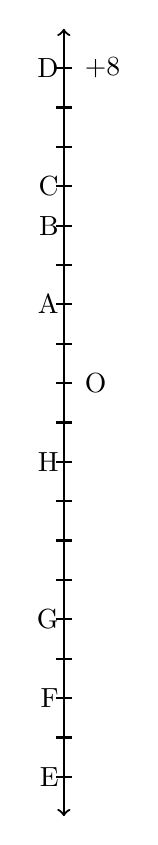
\begin{tikzpicture}
    \draw[thick, <->] (2,-5.5) -- (2,4.5);
    \draw[thick] (1.9,0) -- (2.1,0) node[right=1pt] {O};
    \draw[thick] (1.9,0.5) -- (2.1,0.5);
    \draw[thick] (1.9,-0.5) -- (2.1,-0.5) ;
    \draw[thick] (1.9,1) -- (2.1,1) node[left=1pt] {A};
    \draw[thick] (1.9,-1) -- (2.1,-1) node[left=1pt] {H};
    \draw[thick] (1.9,1.5) -- (2.1,1.5) ;
    \draw[thick] (1.9,-1.5) -- (2.1,-1.5);
    \draw[thick] (1.9,2) -- (2.1,2) node[left=1pt] {B};
    \draw[thick] (1.9,-2) -- (2.1,-2);
    \draw[thick] (1.9,2.5) -- (2.1,2.5) node[left=1pt] {C};
    \draw[thick] (1.9,-2.5) -- (2.1,-2.5);
    \draw[thick] (1.9,3) -- (2.1,3);
    \draw[thick] (1.9,-3) -- (2.1,-3) node[left=1pt] {G};
    \draw[thick] (1.9,3.5) -- (2.1,3.5);
    \draw[thick] (1.9,-3.5) -- (2.1,-3.5) ;
    \draw[thick] (1.9,4) -- (2.1,4) node[left=1pt] {D}  node[right=1pt] {+8};
    \draw[thick] (1.9,-4) -- (2.1,-4) node[left=1pt] {F};
    \draw[thick] (1.9, -4.5) -- (2.1, -4.5);
    \draw[thick] (1.9, -5) -- (2.1, -5) node[left=1pt] {E};
\end{tikzpicture}
}


\item Find the solution of the following:
\begin{enumerate}
\item (+7) + (-11)
\item (-13) + (+10)
\item (-7) + (+9)
\item (+10) + (-5)
\item (– 217) + (– 100)
\end{enumerate}

\item Find the sum
\begin{enumerate}
\item (– 7) + (– 9) + 4 + 16
\item (37) + (– 2) + (– 65) + (– 8)
\end{enumerate}

\item Fill in the blanks with $>, <$ or $=$ sign.
\begin{enumerate}
\item $(– 3) + (– 6)  \ \square \  (– 3) – (– 6)$
\item $(– 21) – (– 10)  \ \square \  (– 31) + (– 11)$
\item $(– 25) – (– 42) \ \square \ (– 42) – (– 25)$
\end{enumerate}

\item Fill in the blanks
\begin{enumerate}
\item $(– 8) + \ \square \ = 0$
\item $13 + \ \square \ = 0$
\item $\ \square \ – 15 = – 10$
\item $(– 4) + \ \square \ = – 12$
\end{enumerate}

\item Find
\begin{enumerate}
\item (– 7) – 8 – (– 25)
\item (– 13) + 32 – 8 – 1
\item (– 7) + (– 8) + (– 90)
\item 50 – (– 40) – (– 2)
\end{enumerate}

\item Between 1 and 20 (including both of them) write 
\begin{enumerate}
 \item all even numbers
 \item all odd numbers
 \item all prime numbers
 \item all composite numbers
\end{enumerate}

\item Find the prime factorization for:
(a) $30 \quad$ (b) $60 \quad$ (c) $72 \quad$ (d) $84 \quad$ (e) $210 \quad$

\item
\begin{enumerate}
 \item List the common prime factors of 256 and 156.
 \item Shreya has two tarps, 84 inches and 96 inches wide. She wants to cut them into strips of equal width as wide as possible. 
 What is the greatest width she can cut?
\end{enumerate}

\item 
\begin{enumerate}
\item Compute Highest Common Factors (HCF) of following pairs:

	(a) $24, 32 \quad$ (b) $15, 225 \quad$  (c) $28, 35 \quad $ (d) $1024, 1020$
	
\item Compute Least Common Multiples (LCM) of following pairs:

	(a) $3, 4 \quad$ (b) $12, 16 \quad $ (c) $21, 15 \quad $ (d) $13, 169$ 
\end{enumerate}



\end{enumerate}


%\vspace*{0.2cm}
%\begin{center}
%{\bf ************************************}
%\end{center}

\end{document}